\chapter{Background}
\label{ch:background}

\section{Steganography}

Steganography is the practice of concealing information within other information.

An example of where this is used is in the prisoners problem, outlined by Simmons (1984) \cite{SIMMONS}, where two prisoners, Alice and Bob, are being held in separate cells. The warden, Walter, of the prison knows that Alice and Bob are likely to try and plot an escape, but Walter cannot prevent their communication until he has proof. Walter tells the prisoners that he will allow them to communicate, but all messages will first be read by him. Alice and Bob must communicate in a way that walter cannot understand, without raising suspicion of the existance of a hidden message. This is where steganography comes in, Alice and Bob could use a technique such as the first letter of each line are combined to make a message (stegotext), it is important that the message read by Walter (covertext) is not suspicious.

There are two types of Warden that can exist, a passive warden and an active warden. The passive warden will not alter the content of the message, but will attempt to detect and prevent hidden communication in a message, whereas an active warden will alter the message in an attempt to spoil any unknown hidden communications, in the prison example Walter could reword the the message so the meaning remains, but the implicit message is lost \cite{aSoCaSaAWA}

A good example of an active warden comes from a tale from World War I, where a cablegram was placed on a censors desk reading "Father is dead", the censor was suspicious and thus rewrote it to say "Father is deceased", shortly after a response was received saying "Is Father dead or deceased?" \cite{TCTSoSW}. This shows the clear benefits to using an active warden, however it does come at a cost, the warden must take the time to analyse the message and alter it, which is costly in real time communication systems.

\section{Digital Steganography}

Digital steganography is a form of steganography that uses digital media as the covertext, the benefit to this is the nature of digital media. This opens up many possibilities in terms of the covertext, for example, a digital image can be used as the covertext, and the stegotext can be hidden in the least significant bits of the image. This is known as Least Significant Bit (LSB) steganography, and is a popular method of digital steganography \cite{AESTfHD}.

In a traditional image this is simply not possible, and highlights the effectiveness of using digital media as the covertext. This is not limited to images, it can be applied to any digital media, such as audio, video, and text. This is the focus of this paper, as the covertext will be the TCP/IP stack, and the stegotext will be hidden in the protocols of the stack.

Another benefit to using digital steganography is the ability to use more complex encoding techniques, and permit asymmetrical encryption to create secure steganographic systems, Hughes (2000) \cite{SaW} defines this as "A system where an opponent who understands the system, but does not know the key, can obtain no evidence (or even grounds for suspicion) that a communication has taken place. ie: no information about the embedded text can be obtained from knowledge of the stego-system".

These secure systems are excellent when working in the TCP/IP stack, because of the nature of the protocols, often using random numbers to have "unique" identifiers, these unique fields can hold encrypted stegotext without raising suspicion, as the fields are expected to be random.

\section{Covert Channels}

The TCP/IP stack is a set of protocols that define how devices communicate over the internet.

The protocols have various fields that hold information about a packet and its contents, these fields can be manipulated to hold stegotext, and thus create a covert channel. The fields used in these covert communications are often required for legitmate communications, which makes the detection and prevention of these channels difficult.

In this paper I will implement three exisiting "static" covert channels:

\subsection{IP Identification Field}

The IP Identification stores "An identifying value assigned by the sender to aid in assembling the fragments of a datagram" \cite{rfc791}, since this value is unique, it is essentially random, this can be used to embed bits \cite{EoIICCA}, making it a good candidate for our secure steganographic system.

Another benefit is the volume of IPv4 traffic on the internet, as of 2022, 30-40\% of end user traffic is IPv6 \cite{I10YO} which means that the majority of traffic is IPv4. This high frequency of traffic in combination with sixteen encodable bits of the identification field allows for an high bandwidth channel, while still maintaining a high quality of covertness.

The short-comings of this channel are outlined in \cite{rfc6864}, where it states "the [identification] field's value is [to be] defined only when fragmentation occurs", this means an active warden could set the identification field to a constant value, thus preventing the use of this channel. This of course could be avoided by using fragmenting the packets, however this is less common and would raise suspicion. This is not a concern when dealing with passive wardens, as they will not alter the packets.

\subsection{TCP Acknowledgement Field}

The TCP Acknowledgement field can be exploited using via the three-way handshake of the TCP protocol, It works because a TCP server will respond to an intial connection request (SYN) that has defined an Initial Sequence Number (ISN), with an ackowledgement (SYN-ACK or SYN-RST (Depending on the status of the port)) that has an acknowledgement number equal to the ISN + 1.

This process can be abused by spoofing the sending address of the client (as the intended covert receiver), and sending a SYN packet with data encoded as the ISN, the server will then respond to the spoofed address (not the orignal sender) with a SYN-ACK packet that has the data encoded as the acknowledgement number. \cite{CCitTCPIPPS}

\begin{figure}[H]
    \centering
    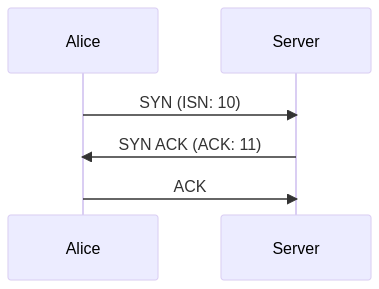
\includegraphics[width=0.8\textwidth]{fig/TCPACKNormal.png}
    \caption{Normal TCP three-way handshake}
    \label{fig:TCPACKNormal}
\end{figure}

\begin{figure}[H]
    \centering
    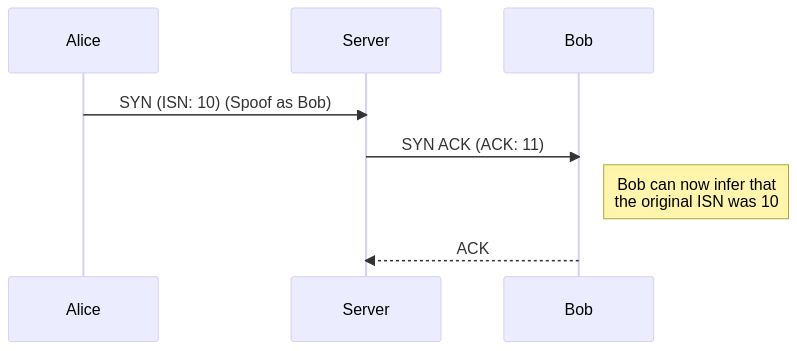
\includegraphics[width=0.8\textwidth]{fig/TCPACKCC.png}
    \caption{TCP three-way handshake with covert channel}
    \label{fig:TCPACKCC}
\end{figure}


By spoofing the address to the recipient, an observing warden will only see communication between the recipient and the server, they will not know the packet actually originated from the sender. This makes it harder to determine if a covert channel is being used, and which systems are involved.

In additon to this, the TCP protocol is used in a large proportion of internet traffic, and its thirty two bit capacity allows gives this channel a very high bandwidth.

The ISN generator is bound to "a (possibly fictious) 32-bit clock that increments roughly every 4 microseconds" \cite{Trfc793}, since the clock is a client-side clock, it is essentially random to an observer, for the first communication. However, a warden could possibly track the allocation of ISNs and determine that a covert channel is likely.

This channel also leaves a trail of failed / incomplete handshakes, as a consequence of not performing the actual handshake. This can raise flags in wardens that are monitoring the network, and thus make the channel less covert. As a further note, this channel is only possible when the spoofed address is in the same subnet as the recipient, otherwise the packet will be dropped leaving the network. 

\subsection{ARP Beaconing}

The Address Resolution Protocol (ARP) is used to map IP addresses to MAC addresses of devices, as outlined in \cite{Arfc826}. When trying to resolve an address, the resolver must broadcast the request to all hosts on the network, as it doesn't know what its physical address is, and await a response.

This leaves the address (that the resolver is trying to determine the physical address of) available for encoding. A limitation here is that the encoded address must be be on the same network, in a /24 subnet, this leaves only a single byte of data available for encoding, reducing the original capacity by 75%.

Requests sent to 'dead' hosts, can raise suspicions in aware wardens, who understand the environment they are operating within \cite{CCUARP}. The redeeming quality of this channel is that, because of the broadcasting nature of the medium, the sender does not need to know the address of the recipient. ARP also play an integral role in network communication, and thus is very unlikely to be blocked by a warden.
